\documentclass[11pt]{report}
\usepackage[utf8]{inputenc}
\usepackage[greek]{babel}
\usepackage{tikz} 
\usepackage{listings}
\newcommand{\en}{\selectlanguage{english}}
\newcommand{\gr}{\selectlanguage{greek}}
\usepackage{fancyhdr}
\usepackage{amsmath}
\pagestyle{plain}
\fancyhf{}
\fancyhead[R]{\leftmark \gr ΛΕΚΚΑΣ ΓΕΩΡΓΙΟΣ ΑΜ:1067430 , ΠΑΠΑΝΙΚΟΛΑΟΥ ΠΑΝΑΓΙΩΤΗΣ ΑΜ:1067431 }
\fancyhead[LO]{\rightmark }
\fancypagestyle{plain}{}
\usepackage{graphicx}
\usepackage{amssymb}
\usepackage{geometry}
\geometry{
	a4paper,
	total={170mm,257mm},
	left=20mm,
	top=20mm,
}
\usepackage{subfig}

\title{\textbf{3o  {\en PROJECT} ΑΠΟΚΕΝΤΡΩΜΕΝΟΣ ΥΠΟΛΟΓΙΣΜΟΣ \& ΜΟΝΤΕΛΟΠΟΙΗΣΗ}}
\author{\gr ΛΕΚΚΑΣ ΓΕΩΡΓΙΟΣ ΑΜ:1067430  Έτος 5ο\\ \\ \gr ΠΑΠΑΝΙΚΟΛΑΟΥ ΠΑΝΑΓΙΩΤΗΣ ΑΜ:1067431  Έτος 5ο\newline}
\date{}
\cfoot{\thepage}
\begin{document}
	\maketitle	
	\thispagestyle{fancy}
	\tableofcontents
	\pagestyle{plain}
	\begin{itemize}
		\item[A.] \gr Θεωρητική Άσκηση 1 
		\item[Β.] \gr Θεωρητική Άσκηση 2
		\item[Γ.] \gr Θεωρητική Άσκηση 3
		\item[Δ.] \gr Προγραμματιστική Άσκηση 1
		\item[Ε.] \gr Προγραμματιστική Άσκηση 2
		
	\end{itemize}
	\pagebreak 
	\section*{\gr \textbf{Α.Θεωρητική Άσκηση 1}}
	
	\gr Οι μεταβλητές του συστήματος είναι οι {\en x1 , x2} και οι οποίες σε μορφή διανύσματος γράφονται ως εξής: $\begin{bmatrix} x1 \\ x2 \end{bmatrix}$ .\\ 
	
	\textbf{1.} Οπότε το μητρώο Α είναι το εξής : A = $\begin{bmatrix} 1 & 0 \\ a & (1-a) \end{bmatrix}$ .\\ \\ Ένα μητρώο είναι στοχαστικό ως προς τις γραμμές όταν το άθροισμα των στοιχείων της κάθε γραμμής είναι ίσο με 1. Πράγματι στο μητρώο Α παρατηρούμε πως $1 + 0 = 1$ και $\alpha + (1- \alpha) = 0$ . \textbf{Επομένως το μητρώο Α είναι στοχαστικό ως προς τις γραμμές.} \\ \\
	
	\textbf{2}. Για να υπολογίσουμε τις ιδιοτιμές και τα ιδιοδιανύσματα του μητρώου Α θα χρησιμοποιήσουμε τους τύπους:  \boldmath {$\det(A - \lambda*I) = 0$} όπου $\lambda$ οι ιδιοτιμές και $I$ το ταυτοτικό μητρώο , \boldmath{$(A - \lambda*I)*x = 0$} . \\ \\
	Συνεπώς έχουμε: \unboldmath{$(A - \lambda*I)$ = $\begin{bmatrix} 1 & 0 \\ a & (1-a) \end{bmatrix}$ - $\lambda*\begin{bmatrix} 1 & 0 \\ 0 & 1 \end{bmatrix}$ = $\begin{bmatrix} 1-\lambda & 0 \\ a & (1-a-\lambda) \end{bmatrix}$ }. \\ \\
	Η ορίζουσα του Α είναι : $\det(A - \lambda*I)$ = $(1 - \lambda)*(1- a - \lambda)$ , οπότε λύνοντας το $\det(A - \lambda*I) = 0$ οι ιδιοτιμές είναι οι : \boldmath{$\lambda = 1$} και \boldmath{$\lambda = 1 - a$}. \\
	Στη συνέχεια για να υπολογίσουμε τα ιδιοδιανύσματα , θα χρησιμοποιήσουμε τον τύπο \unboldmath{$(A - \lambda*I)*\begin{bmatrix} x1 \\ x2 \end{bmatrix}$ = $\begin{bmatrix} 0 \\ 0 \end{bmatrix}$} . \\ \\
	
	Για $\lambda = 1$ έχουμε : $\begin{bmatrix} 0 & 0 \\ a & -a \end{bmatrix}$ * $\begin{bmatrix} x1 \\ x2 \end{bmatrix}$ = $\begin{bmatrix} 0 \\ 0 \end{bmatrix}$ $\Rightarrow$ \boldmath{$\begin{bmatrix} x1 \\ x2 \end{bmatrix}$ = $\begin{bmatrix} 1 \\ 1 \end{bmatrix}$}   (1{\scriptsize 0} ιδιοδιάνυσμα) , \\ \\
	
	Για \unboldmath{$\lambda = 1- a$ έχουμε : $\begin{bmatrix} a & 0 \\ a & 0 \end{bmatrix}$ * $\begin{bmatrix} x1 \\ x2 \end{bmatrix}$ = $\begin{bmatrix} 0 \\ 0 \end{bmatrix}$ $\Rightarrow$} \boldmath{$\begin{bmatrix} x1 \\ x2 \end{bmatrix}$ = $\begin{bmatrix} 0 \\ 1 \end{bmatrix}$}   (2{\scriptsize 0} ιδιοδιάνυσμα)\\ \\ \\
	
	\textbf{3}. To κατευθυνόμενο διάνυσμα {\en G} προκύπτει από το μητρώο Α και συγκεκριμένα απο τη μελέτη των στοιχείων του και τη ταύτιση τους ως μεταβάσεις από τον ένα κόμβο στον άλλο.\\ \\
	Συνεπώς το κατευθυνόμενο γράφημα {\en G} είναι το εξής: \\ \\
	
		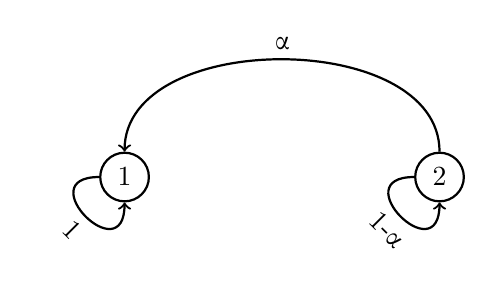
\begin{tikzpicture}[node distance={40mm}, thick, main/.style = {draw, circle}] 
		\node[main] (1) {$1$};
		\node[main] (2) [right of=1] {$2$};	
		
		\draw[->] (1) to [out=180,in=270,looseness=5] node [midway,below,sloped] {1} (1);
		\draw[->] (2) to [out=90,in=90,looseness=1] node [midway,above,sloped] {a} (1);
		\draw[->] (2) to [out=180,in=270,looseness=5] node [midway,below,sloped] {1-a} (2);
		\end{tikzpicture} \\ \\
	Όσον αφορά τη συνεκτικότητα του γραφηματος, το γράφημα είναι \textbf{ασθενώς συνεκτικό} καθώς δεν υπάρχει διαδρομή από τη κορυφή 1 στη κορυφή 2. Για να ήταν ισχυρά συνεκτικό θα έπρεπε να υπήρχε διαδρομή από και προς όλες τις κορυφές του γραφήματος. \\ \\
	
	\textbf{4}. Ο αλγόριθμος ως συνάρτηση των αρχικών τιμών των παικτών συγκλίνει κάθε φορά στο {\en x1}.
	
	\pagebreak 
	\section*{\gr \textbf{Β.Θεωρητική Άσκηση 2}}
	
	
	
\end{document}